\documentclass[a4paper,11pt]{article}
\usepackage{amsmath,amsthm,amsfonts,amssymb,amscd,amstext,vmargin,graphics,graphicx,tabularx,multicol} 
\usepackage[francais]{babel}
\usepackage[utf8]{inputenc}  
\usepackage[T1]{fontenc} 
\usepackage{pstricks-add,tikz,tkz-tab,variations}
\usepackage[autolanguage,np]{numprint} 

\setmarginsrb{1.5cm}{0.5cm}{1cm}{0.5cm}{0cm}{0cm}{0cm}{0cm} %Gauche, haut, droite, haut
\newcounter{numexo}
\newcommand{\exo}[1]{\stepcounter{numexo}\noindent{\bf Exercice~\thenumexo} : \marginpar{\hfill /#1}}
\reversemarginpar


\newcounter{enumtabi}
\newcounter{enumtaba}
\newcommand{\q}{\stepcounter{enumtabi} \theenumtabi.  }
\newcommand{\qa}{\stepcounter{enumtaba} (\alph{enumtaba}) }
\newcommand{\initq}{\setcounter{enumtabi}{0}}
\newcommand{\initqa}{\setcounter{enumtaba}{0}}

\newcommand{\be}{\begin{enumerate}}
\newcommand{\ee}{\end{enumerate}}
\newcommand{\bi}{\begin{itemize}}
\newcommand{\ei}{\end{itemize}}
\newcommand{\bp}{\begin{pspicture*}}
\newcommand{\ep}{\end{pspicture*}}
\newcommand{\bt}{\begin{tabular}}
\newcommand{\et}{\end{tabular}}
\renewcommand{\tabularxcolumn}[1]{>{\centering}m{#1}} %(colonne m{} centrée, au lieu de p par défault) 
\newcommand{\tnl}{\tabularnewline}

\newcommand{\bmul}[1]{\begin{multicols}{#1}}
\newcommand{\emul}{\end{multicols}}

\newcommand{\trait}{\noindent \rule{\linewidth}{0.2mm}}
\newcommand{\hs}[1]{\hspace{#1}}
\newcommand{\vs}[1]{\vspace{#1}}

\newcommand{\N}{\mathbb{N}}
\newcommand{\Z}{\mathbb{Z}}
\newcommand{\R}{\mathbb{R}}
\newcommand{\C}{\mathbb{C}}
\newcommand{\Dcal}{\mathcal{D}}
\newcommand{\Ccal}{\mathcal{C}}
\newcommand{\mc}{\mathcal}

\newcommand{\vect}[1]{\overrightarrow{#1}}
\newcommand{\ds}{\displaystyle}
\newcommand{\eq}{\quad \Leftrightarrow \quad}
\newcommand{\vecti}{\vec{\imath}}
\newcommand{\vectj}{\vec{\jmath}}
\newcommand{\Oij}{(O;\vec{\imath}, \vec{\jmath})}
\newcommand{\OIJ}{(O;I,J)}


\newcommand{\reponse}[1][1]{%
\multido{}{#1}{\makebox[\linewidth]{\rule[0pt]{0pt}{20pt}\dotfill}
}}

\newcommand{\titre}[5] 
% #1: titre #2: haut gauche #3: bas gauche #4: haut droite #5: bas droite
{
\noindent #2 \hfill #4 \\
#3 \hfill #5

\vspace{-1.6cm}

\begin{center}\rule{6cm}{0.5mm}\end{center}
\vspace{0.2cm}
\begin{center}{\large{\textbf{#1}}}\end{center}
\begin{center}\rule{6cm}{0.5mm}\end{center}
}



\begin{document}
\pagestyle{empty}
\titre{Contrôle : Les opérations et les périmètres }{Nom :}{Prénom :}{Classe}{Date}

\vspace*{0.15cm}

\begin{flushleft}
\begin{tabular}{|m{6.5cm}|m{2.5cm}|m{2.5cm}|m{2.5cm}|m{2.5cm}|}
\hline 
\textbf{Compétences} & \begin{center}
\textbf{Très bonne maîtrise}
\end{center} & \begin{center}
\textbf{Maîtrise satisfaisante}
\end{center}  & \begin{center}
\textbf{Maîtrise faible}
\end{center} & \begin{center}
\textbf{Maîtrise insuffisante}
\end{center} \\ 
\hline 
 Prélever et organiser les informations nécessaires à la résolution de problèmes à partir de supports variés : textes, dessins, schémas, etc &  &  & &\\
\hline
Reconnaitre et distinguer des problèmes relevant de situations additives, multiplicatives &  &  & & \\ 
\hline
 Calculer avec des nombres décimaux, de manière exacte ou approchée, en utilisant des stratégies ou des techniques appropriées (mentalement, en ligne, ou en posant les opérations) &  &  &  &\\ 
\hline 



\end{tabular} 
\end{flushleft}

\vspace*{0.5cm}

Les exercices avec le signe 
\includegraphics[scale=0.3]{trefle.eps} sont à faire directement sur le sujet. Les autres se font sur la copie double.\\

\exo{4.5} 
\includegraphics[scale=0.3]{trefle.eps} Pour chacune des questions, entourer la bonne réponse :

\begin{flushleft}
\begin{tabular}{|c|m{10cm}|c|c|c|}
\hline 
 &  & \textbf{A} & \textbf{B} & \textbf{C} \\ 
\hline 
\textbf{1} & J'achète un pain à 1,75 euros, un croissant à 0,70 euros, un pain au chocolat à 0,90 euros et une brioche à 2,20 euros. Quel billet dois-je donner pour que la boulangère me rende le minimum de monnaie ?
 & 5 euros & 10 euros & 20 euros \\ 
\hline 
\textbf{2} & Un camion transporte 100 palettes.
Chaque palette contient 10 packs de 6 bouteilles d'eau minérale de 1,5 L.
Combien de litres d'eau transporte ce camion ?
 & 6 000 L & 117,5 L & 9 000 L \\ 
\hline 
\textbf{3} & Quelle masse obtient-on quand 
on ajoute 5 g à 2,3 hg ?
 & 2,8 hg	 & 2,35 hg	 & 2,305 hg \\ 
\hline 
\textbf{4} & Quel est le plus lourd : 8,7 kg ou 8 070 dg? & 
8,7 kg	 & 8 070 dg & 	C'est la même masse \\ 
\hline 
\textbf{5} & Le nombre 4 35$\star$ a un chiffre inconnu. Pourtant, on sait qu'il est multiple de 9. 
Donc le chiffre inconnu (remplacé par $\star$) peut être égal  à …
 & 6 & 1 & 3 \\ 
\hline 
\textbf{6} & Si le diviseur est 9, si le reste est 13  et si le quotient est 5  alors le dividende est … & 58		 & 74 & 122\\ 
\hline 
\end{tabular} 

\end{flushleft}
\vspace*{0.5cm}

\exo{2} Calculer astucieusement les expressions suivantes, en détaillant les étapes de calculs :

\bmul{2}

$B = 24,6 + 3,5 + 7,8 + 5,4 + 2,2 + 6,5 + 19,72 + 10,28 $\\


\columnbreak

$G = 4 \times 3 \times 250 \times 0,6$

\emul

\exo{3} 
\includegraphics[scale=0.3]{trefle.eps} Compléter le tableau avec « oui » ou « non ».\\

\begin{tabular}{|c|c|c|c|c|}
\hline 
 & Divisible par 2 & Divisible par 3  & Divisible par 4  & Divisible par 5  \\ 
\hline 
714 &  &  &  &  \\ 
\hline 
51 120 &  & &  &  \\ 
\hline 
185 &  &  &  &  \\ 
\hline 
\end{tabular} 

\newpage

\vspace*{0.5cm}

\exo{2.5}

\includegraphics[scale=0.7]{exodistance.eps} 

\q Calculer les distances Rouen-St Malo et Amiens-Quimper.\\

\q Quelle distance cherche-t-on quand on propose le calcul suivant :   $610 - (411 +97)$ ?\\

\vspace*{0.5cm}


\exo{2.5}\\
Paula fait des courses avec un billet de 20 euros en poche. Elle achète :\\
- 3 baguettes à 0,97 euro l'une, \\
- 2,7 kg de pommes à 1,50 euros le kg,\\
- 700 g de viande à 12,30 euros le kg.\\

$\rightarrow$  Combien lui reste-t-il après ses achats ? \textit{Faire apparaître les conversions éventuelles et vos calculs.}\\

\vspace*{0.5cm}

\exo{1.5}

\bmul{2}

La figure ci-contre n'est pas représentée en grandeur réelle.\\

$\rightarrow$ Calculer le périmètre de cette figure.\\

\columnbreak

\includegraphics[scale=1]{exoperimetre.eps} 

 \emul

\vspace*{0.5cm}

\exo{3}

A une table ronde de 1,10 m de diamètre, on peut ajouter trois rallonges de 40 cm chacune.
\bmul{2}

\initq \q Calculer, en m, le périmètre de la table ronde sans les rallonges.\\

\q  Calculer le périmètre de la table avec ses trois rallonges.\\

\columnbreak

\includegraphics[scale=1]{exoperimetre2.eps} 

\emul

\q En comptant 60 cm par personne, Félix dit qu'on peut mettre 10 personnes autour de cette table avec rallonges et Annie dit qu'on ne peut en mettre que 9.\\
    Qui a raison ? Pourquoi ?\\



\vspace*{0.5cm}

\exo{} Bonus \\

\initq \q Écrire tous les nombres inférieurs à 115 qui sont à la fois multiples de 2, de 3 et de 5 .\\

\q La tour Montparnasse a une hauteur de 0,209 km. La tour Eiffel la dépasse de 11,5 dam.\\
 Calculer la hauteur, en m, de la tour Eiffel.\\



\end{document}
